% !TeX root = POSTER.tex
\documentclass[25pt, a0paper,
portrait,
% landscape,
margin=2mm, 
innermargin=2mm, 
blockverticalspace=7mm, %distance between upper and lower block
colspace=2mm, %distance between left and right block 
subcolspace=0mm]{tikzposter}
		
% -- Packages --------------------------------------------------------%
\usepackage{amsfonts,amssymb,amsmath,mathtools}
\usepackage{defcmlfont}
\usepackage{tikz,lipsum}

\usepackage[T1]{fontenc}
% \usepackage{lmodern}
% \usepackage[english]{babel}

\usetikzlibrary{positioning}
\usepackage{float}                           % for minipages at Polarization part
\usepackage{caption}                         % no "Figure" in caption
\captionsetup[figure]{labelformat=empty}

\usepackage{psfrag}

% Load figures command: \inputfig [htb]{fig_dir}{fig_label}
\newcommand*{\inputfig}[3][htb]{{
    \def\fps@figure{#1}
    \def\DIR{#2}
    \def\LABEL{#3}
    \graphicspath{{\DIR/}}
    \psfrag{sm}[c][c]{\small \textsc{Scan me}}


\includegraphics[width=0.03\textwidth]{QRcode_ACoM.eps}
}}

\usepackage{fontawesome}
\usepackage{bm}
\usepackage{bigints}
\usepackage{relsize}

\usepackage{accents}

\usepackage{lipsum} 

\usepackage{babel}
\usepackage{hyperref}
\usepackage{cleveref}

\usepackage{mdframed}

% -- Commands --------------------------------------------------------%
% \newcommand{\wall}{\text{w}}
% \newcommand{\interf}{\text{i}}
% \newcommand{\phase}{k}	
% \newcommand{\liquid}{\ell}
% \newcommand{\steam}{g}
% \newcommand{\out}{\text{out}}
% \newcommand{\tr}{{\mathsf T}}
\newcommand{\WAsigma}{\prescript{\prescript{\mathcal{W}}{}{\!\!\!\mathcal{A}}}{}{\!\sigma}}
\newcommand{\WABsigma}{\prescript{\prescript{\mathcal{W}}{}{\!\!\!\mathcal{A}}}{}{\!\boldsymbol{\sigma}}}

% Mathematic sets
\newcommand{\mbR}{\mathbb{R}}
\newcommand{\mbC}{\mathbb{C}}

% mathcals
\newcommand{\mcA}{\mathcal{A}}
\newcommand{\mcB}{\mathcal{B}}
\newcommand{\mcC}{\mathcal{C}}
\newcommand{\mcD}{\mathcal{D}}
\newcommand{\mcE}{\mathcal{E}}
\newcommand{\mcO}{\mathcal{O}}
\newcommand{\mcS}{\mathcal{S}}
\newcommand{\mcT}{\mathcal{T}}
\newcommand{\mcV}{\mathcal{V}}
\newcommand{\mcW}{\mathcal{W}}

% -- Title, Author, Institute --------------------------------------------------------%
% \title{
% \begin{minipage}{0.22\textwidth}
% 	
\includegraphics[width=1.02\textwidth]{./floats/logos/siam_siamcse23.eps}
% \end{minipage}
% \hfill
% \begin{minipage}{0.46\textwidth}
% 	\begin{flushleft}
% 		{\bfseries Next-generation all-solid-state battery}
% 	\end{flushleft}
% 	% \author{\underline{Tuan Vo}$^{\text{a,b}\,\dagger}$, Claas Hüter$^{\text{b}}$, Stefanie Braun$^{\text{a}}$, Manuel Torrilhon$^{\text{a}}$}
% 	% {\normalsize \underline{Tuan Vo}$^{\text{a,b}\,\dagger}$, Claas Hüter$^{\text{b}}$, Stefanie Braun$^{\text{a}}$, Manuel Torrilhon$^{\text{a}}$}
% \end{minipage}
% \hfill
% \begin{minipage}{0.22\textwidth}
% 	% \begin{flushleft}
% 		
\includegraphics[width=1.02\textwidth]{./floats/logos/rwth_acom_en_cmyk_fzj_gap.eps}
% 	% \end{flushleft}
% \end{minipage}
% }
\title{\scshape Next-generation all-solid-state battery (\#ASSB)}
\author{
	\underline{Tuan Vo}$^{\text{a,b}\,\dagger}$, Claas Hüter$^{\text{b}}$, Stefanie Braun$^{\text{a}}$, Manuel Torrilhon$^{\text{a}}$\\
\normalsize vo@acom.rwth-aachen.de}
\author{\underline{Tuan Vo}$^{\text{a,b}\,\dagger}$, Claas Hüter$^{\text{b}}$, Stefanie Braun$^{\text{a}}$, Manuel Torrilhon$^{\text{a}}$}
\institute{\large
$\prescript{a}{}{}$Department of Mathematics, Applied and Computational Mathematics (ACoM), 
RWTH Aachen University, Schinkelstraße 02, 52062 Aachen, Germany\\
$\prescript{b}{}{}$Institute of Energy and Climate Research (IEK-2), 
Forschungszentrum Jülich, Wilhelm-Johnen-Straße, 52428 Jülich, Germany
}

% \titlegraphic{
\includegraphics[height=6cm]{./figs/FZJ_only.pdf} \hfill 
\includegraphics[height=6cm]{./figs/rwth_mathcces_bild_rgb_only.pdf} }
% \titlegraphic{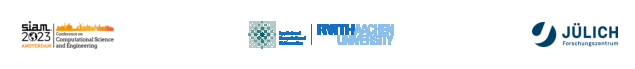
\includegraphics[width=0.3\textwidth]{./floats/logos/rwth_acom_en_cmyk_siamcse23_fzj_gap.eps}}

% \renewcommand{\familydefault}{\sfdefault} % Change font family

\bibliographystyle{plain}

\newcommand{\newcaption}[2]{\parbox{#1}{\centering{\small \it #2\par}}\normalsize}

% -- Predefined Colors and Themes ---------------------- %
% Choose THEME:  Default, Basic, Rays, Simple, Envelope, Wave, Board, Autumn, Desert,
% Explanation THEME: Default(gray+blueBC), Basic(green light), Rays(blue), 
% Simple(red), Envelope(Bluefancy), Wave(Bluefancy2), Board(Bluelight), Autumn(squarebox+bluebrown), Desert(squarebox+bluebrown2),
\usetheme{Default}

\useblockstyle[titleinnersep=0.7mm]{Default}    % change default parameter for title inner sep
% Choose COLOR STYLE:  Default, Blue, BlueGray, BlueOrange, BlueViolet, DarkBlue, GrayBlue, GrayLightblue, GrayRed, Green, GreenOrange, YellowRed
%\definecolor{main}{HTML}{0080FF}
%\definecolor{sub}{HTML}{8CDBFF}
%\usecolorstyle[colorOne=sub, colorTwo=main]{Default}
%     
% To-do-list
% 1. Rotate 3 Matlab figures
% 2. Explain for symbols
% 3. Comparison results Numa vs. Ana
% 4. Structure tensor math?
% 5. Next-generation ASSB typing master balance?
% 6. ASSB nucleation figure settings nicely again
% 7. Numerical figures nice again 4x about evolution?
% 8. Boundary settings nicely again
% 9. Scan me a bit to the right
% ---------------------------------------------------------------------------------------------------------------- %
\begin{document}
% Title block
\maketitle[width=800mm]
% \block{}{
% 	d
% }
% ---------------------------------------------------------------------------------------------------------------- %
\block{\bfseries Mathematical modelling for the next-generation All-solid-state batteries: Nucleation $\text{(SE|SSE)}^{\!(*)}$-interface}{
	\begin{minipage}{0.55\textwidth}
		\begin{minipage}{0.5\textwidth}
			\begin{mdframed}
				\textbf{Rechargeable Lithium-ion battery} (LIB)
				is at the heart of every electric vehicle (EV), portable electronic device,
				and energy storage system \cite{vo2018}. 
				Nowadays, LIBs enable human life more efficient 
				and help to solve global environment issues thanks to EVs' zero emission.
				However, conventional LIB (c-LIB) is sensible to temperature and pressure, 
				hence, flammable and explosive. 
				This bottleneck is mainly due to liquid-based electrolyte in c-LIBs.
			\end{mdframed}
		\end{minipage}
		% \hfill
		\begin{minipage}{0.49\textwidth}
			\begin{mdframed}
				\textbf{All-solid-state battery} (ASSB) is 
				one of promising candidates to overcome bottlenecks of c-LIBs. 
				Thanks to solid-state electrolyte (SSE),
				% e.g. SSE made of the highly ionic-conductive polycrystalline LLZO, 
				ASSB is highly stable towards temperature and pressure. 
				Nevertheless, metallic Li-dendrite 
				triggered at (SE|SSE)-interface is the main drawback 
				as these dendritic threads extrapolate into grain boundary network of SSE, 
				causing crevice, degradation of ionic conductivity,
				and the probability of short-circuit.
			\end{mdframed}
		\end{minipage}
		%
		\begin{mdframed}
			\textbf{Next-generation All-solid-state battery} (ng-ASSB)
			% should, consequentially, be able to cope with 
			% micro-dendritic threads at the (SE|SSE)-interface, 
			% and hence, 
			% to foresee nucleation points caused by propagations 
			% of 
			% these dendrites, 
			% when possible.	
			with a consideration of nucleation criterion defined by
			% \begin{align*}
			% 	 & \rho\,
			% 	\partial^2_{t^2}
			% 	\bm{u}^{(s)}
			% 	+
			% 	\nabla \cdot
			% 	\Big(
			% 	\accentset{\scriptstyle 4}{\mathbb{C}}^{f^{\mathbb{D}(\Omega)}_{(\lambda,\mu)}}
			% 	:\nabla\Bu^{(s)}
			% 	\Big)
			% 	+
			% 	\rho\nabla V_{e}
			% 	= \textbf{0},                                                                                                                                                                                                                                                               \\
			% 	%--------------------------------
			% 	\text{s.t.}\quad
			% 	 & a_{\text{Griffith}} := a^{*} = \arg\min_{a\in\mathbb{R}}{\bigintsss\!\!\!\!\!\!\bigintsss\!\!\!\!\!\!\bigintsss_{\Omega} f(a,\bm{u};\lambda,\mu,\bm{d}\otimes\bm{d}) \, d\Omega - \bigintsss\!\!\!\!\!\!\bigintsss_{\Gamma} f(a;\gamma) \, d\Gamma}\Bigg|_{\bm{u}^{(s)}}
			% \end{align*}
			\begin{align*}
				a_{\text{Griffith}} := a^{*} = \arg\min_{a\in\mathbb{R}}{\bigintsss\!\!\!\!\!\!\bigintsss\!\!\!\!\!\!\bigintsss_{\Omega} f(a,\bm{u};\lambda,\mu,\bm{d}\otimes\bm{d}) \, d\Omega - \bigintsss\!\!\!\!\!\!\bigintsss_{\Gamma} f(a;\gamma) \, d\Gamma}\Bigg|_{\bm{u}^{(s)}}
			\end{align*}
			where,
			can help to improve ASSB performance.
		\end{mdframed}
	\end{minipage}%
	\hfill
	\begin{minipage}{0.45\textwidth}
		% \begin{tabular}{|p{\textwidth}}
		% 	This is second part                                                                              \\
		% 	$f(x) = 2x + 3y$ This line may go all along the end and wrap afterwards to the next as seen here \\
		% 	This is a forced next line by ending the previous line 
		% \end{tabular}
		% \inputfig{floats/dendrite_pdirection_battonly}{dendrite_pdirection_battonly}
		\begin{center}
			\inputfig{floats/routine_woTV_spectral}{routine_woTV_spectral}
		\end{center}
	\end{minipage}%
	% \begin{columns}
	% 	\column{0.5}
	% 	Goal:
	% 	\begin{align}
	% 		a_{\text{Griffith}} := a^{*} = \arg\min_{a\in\mathbb{R}}{\bigintsss\!\!\!\!\!\!\bigintsss\!\!\!\!\!\!\bigintsss_{\Omega} f(a,\bm{u};\lambda,\mu,\bm{d}\otimes\bm{d}) \, d\Omega - \bigintsss\!\!\!\!\!\!\bigintsss_{\Gamma} f(a;\gamma) \, d\Gamma}\Bigg|_{\bm{u}^{(s)}}
	% 	\end{align}
	% 	where
	% 	\column{0.5}
	% 	abc
	% 	% \begin{center}
	% 	% 	% \fbox{\inputfig{floats/creviceAiryWestergaard_compare}{creviceAiryWestergaard_compare}}
	% 	% 	\inputfig{floats/dendrite_pdirection_battonly}{dendrite_pdirection_battonly}
	% 	% \end{center}
	% 	\textbf{This poster} is aimed to model the nucleation
	% 	by taking into consideration
	% 	\underline{polarization}, \underline{structural tensor}, 
	% 	\underline{locally non-uniform electric field}, and 
	% 	\underline{Griffith analysis}. 
	% 	\begin{align}
	% 		 & \rho\,
	% 		\partial^2_{t^2}
	% 		\bm{u}^{(s)}
	% 		+
	% 		\nabla \cdot
	% 		\Big(
	% 		\accentset{\scriptstyle 4}{\mathbb{C}}^{f^{\mathbb{D}(\Omega)}_{(\lambda,\mu)}}
	% 		:\nabla\Bu^{(s)}
	% 		\Big)
	% 		+
	% 		\rho\nabla V_{e}
	% 		= \textbf{0},                                                                                                                                                                                                                                                               \\
	% 		%--------------------------------
	% 		\text{s.t.}\quad 
	% 		 & a_{\text{Griffith}} := a^{*} = \arg\min_{a\in\mathbb{R}}{\bigintsss\!\!\!\!\!\!\bigintsss\!\!\!\!\!\!\bigintsss_{\Omega} f(a,\bm{u};\lambda,\mu,\bm{d}\otimes\bm{d}) \, d\Omega - \bigintsss\!\!\!\!\!\!\bigintsss_{\Gamma} f(a;\gamma) \, d\Gamma}\Bigg|_{\bm{u}^{(s)}}
	% 	\end{align}
	% 	where
	% \end{columns}
	% \begin{center}
	% 	\inputfig{floats/dendrite_pdirection_battonly_maths}{dendrite_pdirection_battonly_maths}
	% \end{center}
}
% ---------------------------------------------------------------------------------------------------------------- %
\begin{columns}
	\column{0.34}{
		\block{Interface}{
			\textbf{Interface} between solid electrode and solid-state electrolyte (SE|SSE) 
			taking place at space charge layer (SCL) \cite{braun2015}
			found in ASSBs 
			critically exhibits mechanical and electrochemical instability \cite{hueter2017}. 
			This evidence points directly to the fact that 
			the soft metallic li anode 
			is erroneously prone to triggering dendrites, 
			under cycles of electric charge \& discharge \cite{kim2022}.
			\begin{center}
				\inputfig{floats/maxshear_9figs_456}{maxshear_9figs_456}
			\end{center}
			Distribution:\! ana. max. shear stress $\WAsigma^{\Pi}_{x_1x_2}$ around crack tip $a_{c}$.
		}
	}
	% ---------------------------------------------------------------------------------------------------------------- %
	\column{0.34}
	% ---------------------------------------------------------------------------------------------------------------- %
	\block{Next-generation All-solid-state battery
		% (ng-ASSB)
	}{
		Nucleation taking place at critical dendritic (SE|SSE)-interface
		\begin{center}
			\inputfig{floats/dendrite_pdirection_battonly}{dendrite_pdirection_battonly}
		\end{center}
		Nucleation taking place at critical dendritic (SE|SSE)-interface\\
		Nucleation taking place at critical dendritic (SE|SSE)-interface
		% This phenomenon, notwithstanding, is predicted, quantified, and controlled based on analysing 
		% the multi-scale coupled problem subjected to conditions of Griffith criterion.
		%
		% \begin{center}
		% \fbox{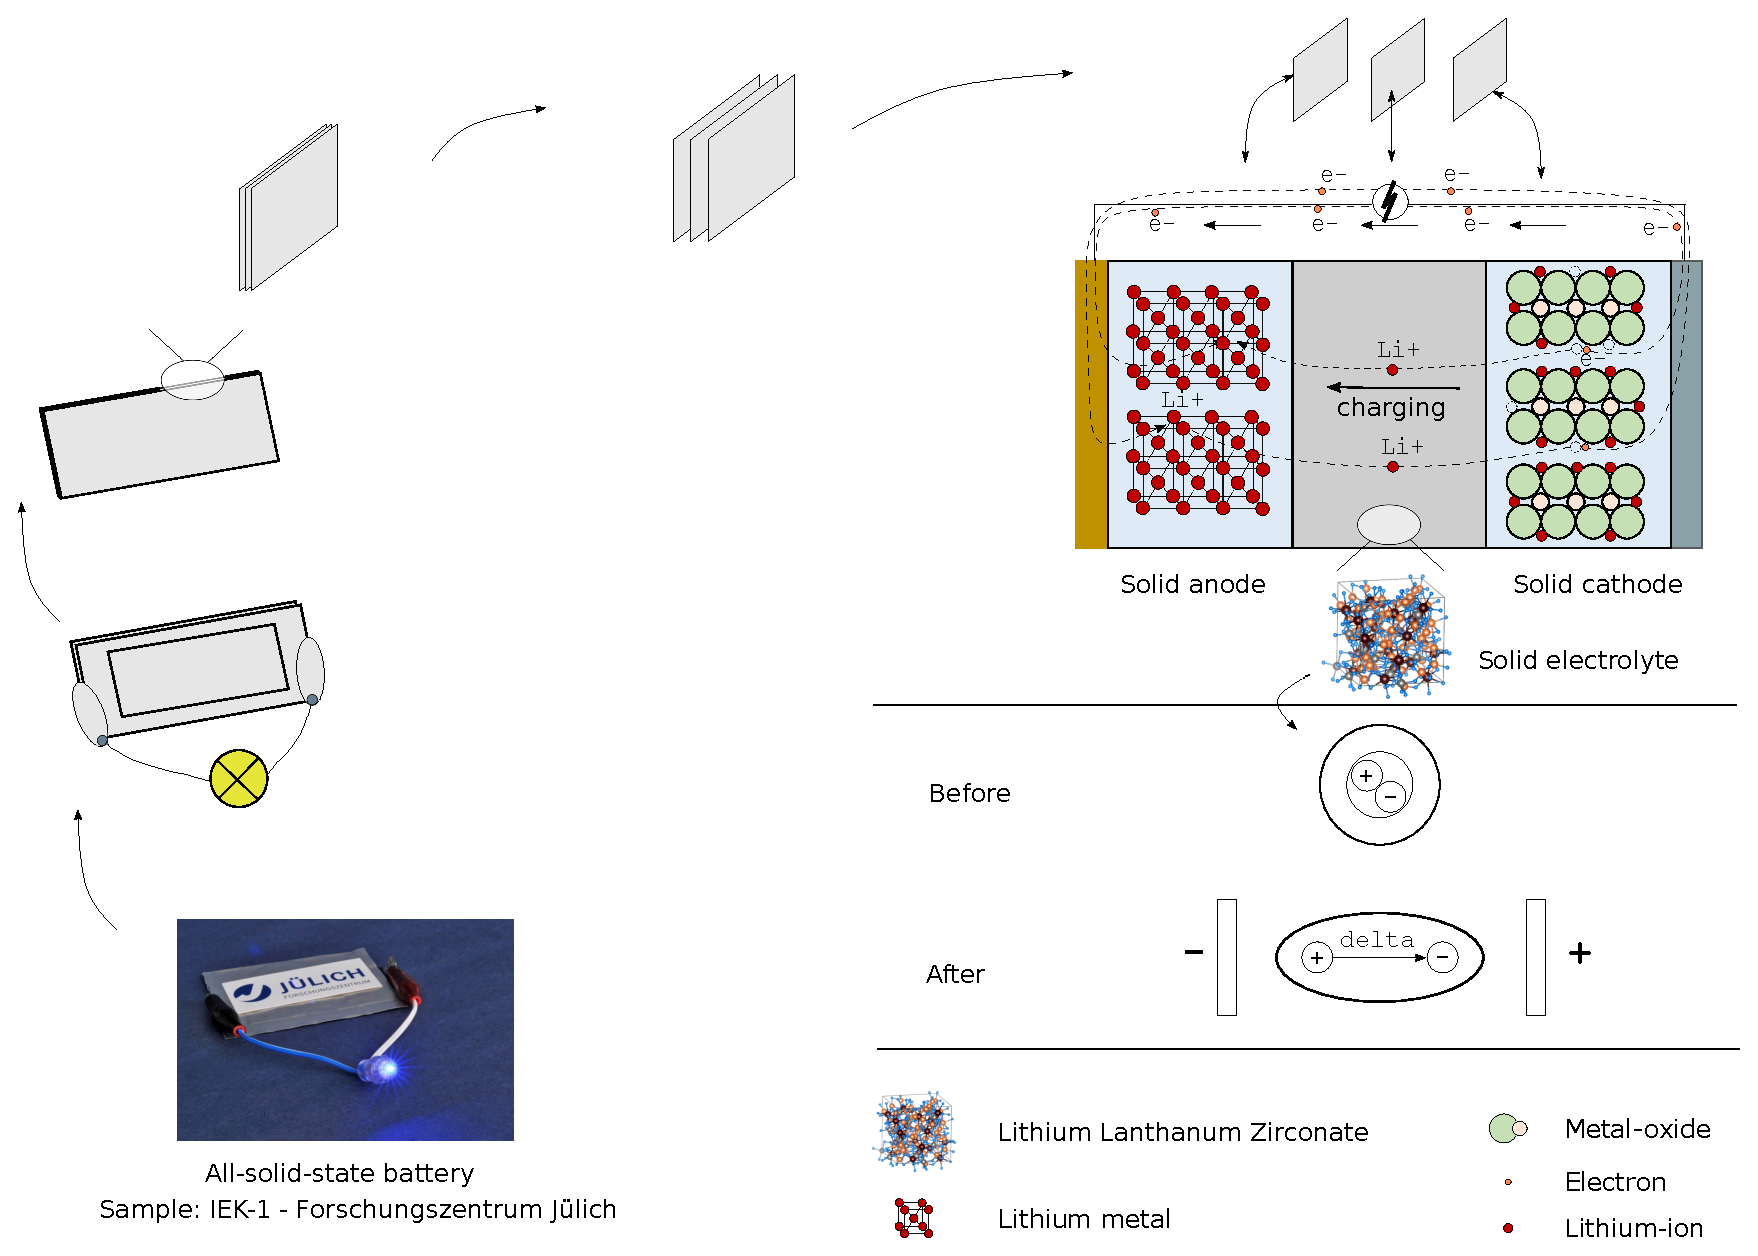
\includegraphics[height=18cm]{./figs/dendrite/dendritetext}}
		% \fbox{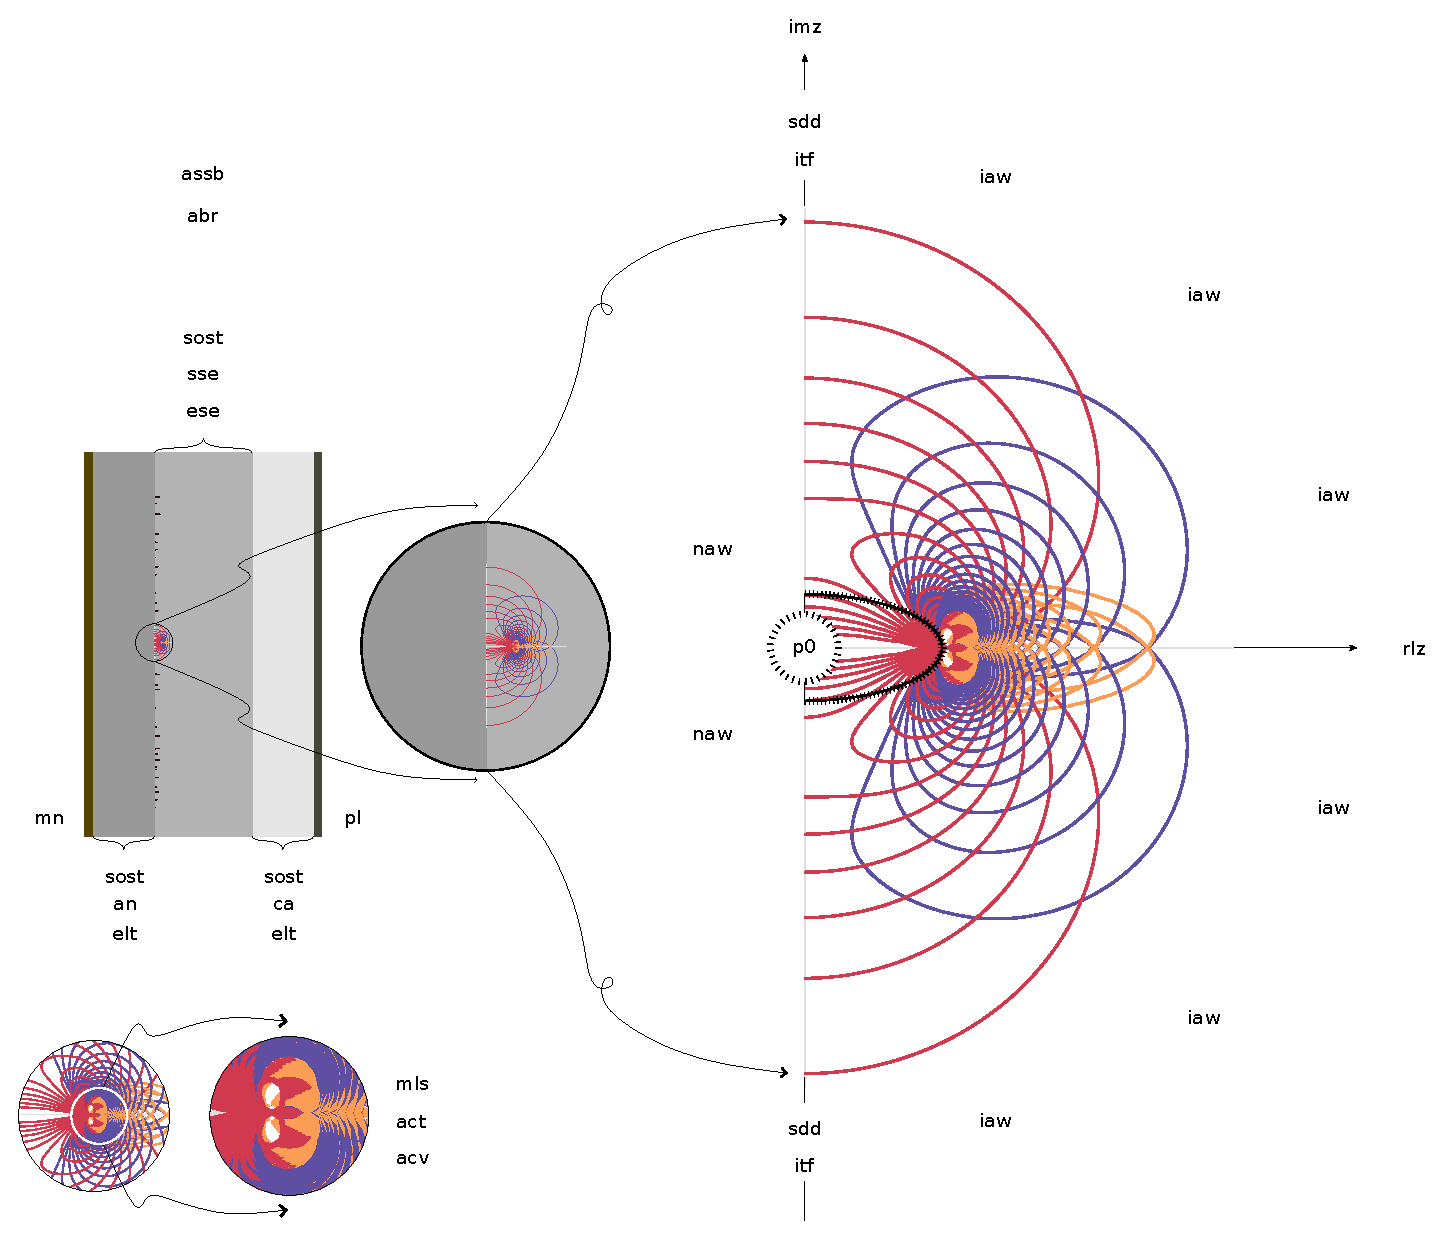
\includegraphics[height=18cm]{./floats/creviceAiryWestergaard_compare/creviceAiryWestergaard_compare.eps}}
		% 	\newcaption{0.8\colwidth}{A sample of a typical all-solid-state battery and its non-scale hierarchical insight into structural layers.}
		% \end{center}
		
		% A typical LIB includes three main components: cathode, anode and electrolyte. 
		% Different types of LIB have a variation of constitutive material composed of battery. 
		% An ASSB means that the three main components are \textbf{all made of solid material}.
	}
	% ---------------------------------------------------------------------------------------------------------------- %
	% \block{Modelling goal: Interface analysis + Numerics}{
	% 	Two main goals to model the solid electrolyte part of the all-solid-state battery is as follows:
	% 	%
	% 	\begin{enumerate}
	% 		\item To capture the \textbf{preferred direction} behaviour of the solid electrolyte due to electric potential.
	% 		\item To satisfy \textbf{thermodynamic consistency}%\cite{braun2015SCL}
	% 		      :
	% 		      \begin{itemize}
	% 			      \item Conservation of mass, linear $\&$ angular momentum and energy for the solid electrolyte.
	% 			      \item Entropy inequality is guaranteed with sharper conditions, which lead to constitutive equation.
	% 		      \end{itemize}
	% 	\end{enumerate}
	% 	\begin{align*}
	% 		a_{\text{Griffith}}:= a^{*}
	% 		= \arg\min_{a\in\mathbb{R}}
	% 		{
	% 			\bigintsss\!\!\!\!\!\!\bigintsss\!\!\!\!\!\!\bigintsss_{\Omega}
	% 			f(a,\bm{u};\lambda,\mu,\bm{d}\otimes\bm{d}) \, d\Omega
	% 			-
	% 			\bigintsss\!\!\!\!\!\!\bigintsss_{\Gamma}
	% 			f(a;\gamma) \, d\Gamma
	% 		}\Bigg|_{\bm{u}^{(s)}}
	% 	\end{align*}
	% }
	% ---------------------------------------------------------------------------------------------------------------- %
	% \block{Continuum physics kinematic}{
	% 	Green-Lagrange strain tensor $\BE$ with respect to \textbf{small} displacement 
	% 	$\partial\Bu/\partial\Bxi = \mathcal{O}(\epsilon), \ \epsilon \ll 1$:
	% 	\begin{align*}
	% 		\BE = \frac{1}{2}(\BF^{\top}\BF -\BI) =\frac{1}{2}\left(
	% 		\frac{\partial\Bu}{\partial\Bxi} + \left( \frac{\partial\Bu}{\partial\Bxi} \right)^{\top}
	% 		+\underbrace{\left( \frac{\partial\Bu}{\partial\Bxi} \right)^{\top}\left( \frac{\partial\Bu}{\partial\Bxi} \right)}_{\text{Neglected}}
	% 		\right) \ \rightarrow \
	% 		\Bvarepsilon := \frac{1}{2}\left(
	% 		\frac{\partial\Bu}{\partial\Bxi} + \left( \frac{\partial\Bu}{\partial\Bxi} \right)^{\top}\right)
	% 	\end{align*}
	% }
	% ---------------------------------------------------------------------------------------------------------------- %	
	% \block{Polarization phenomenon}{
	% 	Due to a source of electric potential pointing from cathode $(+)$ to anode $(-)$ pole, 
	% 	a uniform electric field created has suppressed on 
	% 	the SE occupied between these two poles. Consequently, SE yields to a \textbf{preferred direction}
	% 	under external deformations such as mechanical loading forces.
	% 	% \begin{minipage}{\linewidth}
	% 	% 	\centering
	% 	% 	\begin{minipage}{0.20\linewidth}
	% 	% 		\begin{figure}[H]
	% 	% 			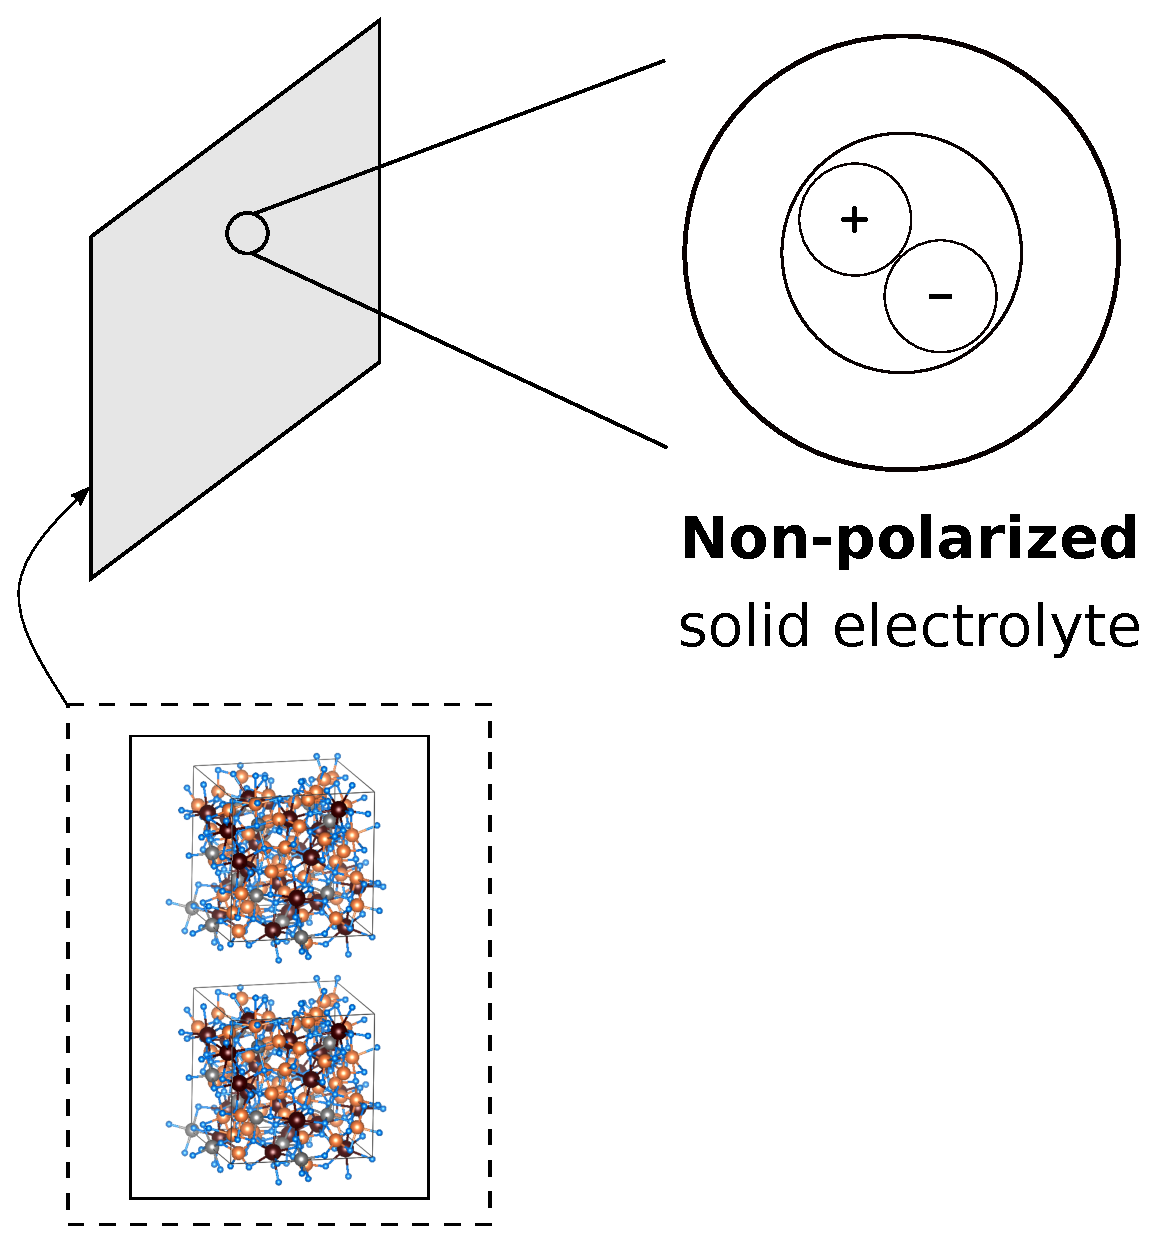
\includegraphics[width=\linewidth]{./figs/polarization/polarizedSEnon}
	% 	% 			%\caption{Non-polarized SE.}
	% 	% 		\end{figure}
	% 	% 	\end{minipage}
	% 	% 	\hspace{0.2\linewidth}
	% 	% 	\begin{minipage}{0.25\linewidth}
	% 	% 		\begin{figure}[H]
	% 	% 			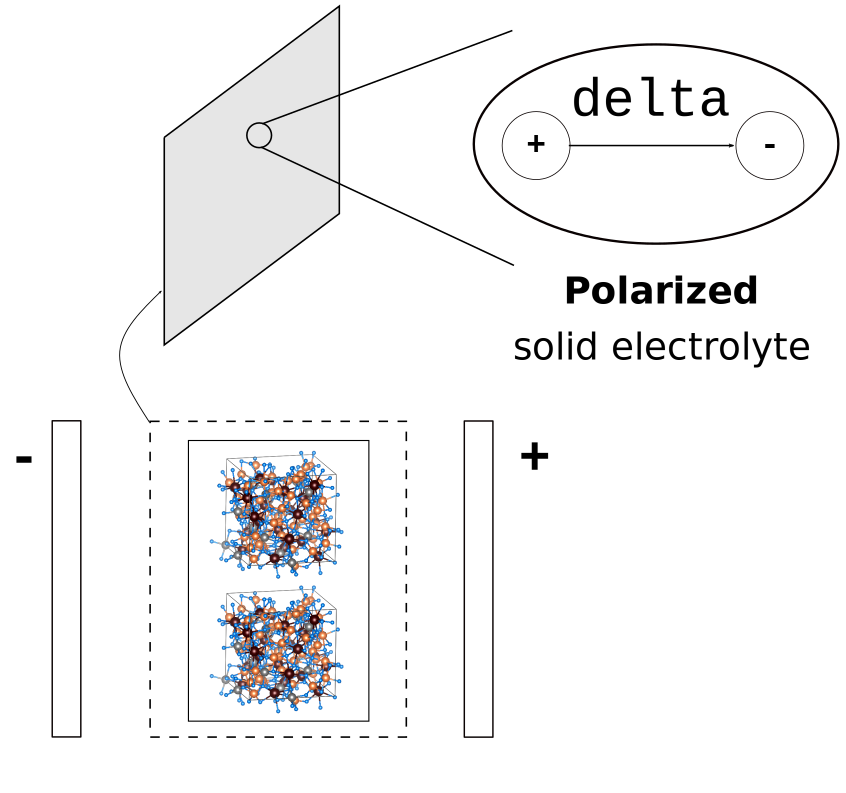
\includegraphics[width=\linewidth]{./figs/polarization/polarizedSE}
	% 	% 			%\caption{Polarized SE.}
	% 	% 		\end{figure}
	% 	% 	\end{minipage}
	% 	% \end{minipage}
	% }
	% ---------------------------------------------------------------------------------------------------------------- %
	% SECOND column
	% ---------------------------------------------------------------------------------------------------------------- %
	\column{0.32}
	\block{Embedded structural-tensor SSE}{
		% \begin{center}
		% 	\inputfig{floats/dendrite_pdirection_battonly}{dendrite_pdirection_battonly}
		% \end{center}
		Polycrystalline garnet-typed SSE 
		such as LLZO 
		exhibit grain boundaries and various sizes 
		and shapes of grains under microscopic observation.
		Therefore, this type of microstructure distinctively leads to 
		nuance destruction of ceramic-like materials.
		\begin{center}
			\inputfig{floats/dendrite_2parts_nospl_split}{dendrite_2parts_nosample_split}
		\end{center}
		Consequentially, dendrites contribute to 
		degradation of ionic conductivity
		and trace along grain boundaries in SSE.
		% \begin{center}
		% 	\inputfig{floats/dendrite_pdirection_battonly}{dendrite_pdirection_battonly}
		% \end{center}
		% \inputfig{floats/efield}{efield}
		% \inputfig{floats/maxshear_9figs_456}{maxshear_9figs_456}
		% \begin{center}
		% 	\inputfig{floats/creviceAiryWestergaard_compare}{creviceAiryWestergaard_compare}
		% 	% \inputfig{floats/dendrite_pdirection_battonly}{dendrite_pdirection_battonly}
		% \end{center}
		% \begin{itemize}
		% 	\item Local balance laws governing the infinitesimal elasticity embedded structural tensor:
		% 	      \begin{align*}
		% 		       & \text{Balance of mass}             &  & \dot{\rho} + \rho{\ \rm div}\Bv = 0                             \\
		% 		       & \text{Balance of linear momentum}  &  & \rho\dot{\Bv} = {\rm div}\Bpi + \rho\Bb                         \\
		% 		       & \text{Balance of angular momentum} &  & \Bpi^{\top} = \Bpi                                              \\
		% 		       & \text{Balance of energy}           &  & \rho\dot{e} = \Bpi : \dot{\Bvarepsilon} + \rho r - {\rm div}\Bq
		% 	      \end{align*}
		
		% 	\item Entropy inequality
		% 	      \begin{align*}
		% 		      \rho\calD := \Bpi :\dot{\Bvarepsilon}  -\rho\eta\dot{\theta}- \rho\dot{\Psi} -\frac{1}{\theta}\Bq\cdot\nabla\theta \geq 0 
		% 	      \end{align*}
		
		% 	\item Mathematical model:
		% 	      \begin{align*}
		% 		       & \text{PDE}                   &  & \pi_{ij,j} + \rho b_{i} = 0                                                                                      \\
		% 		       & \text{Kinematic relation}    &  & \varepsilon_{kl} = \frac{1}{2}\left(\frac{\partial u_k}{\partial x_l} + \frac{\partial u_l}{\partial x_k}\right) \\
		% 		       & \text{Constitutive relation} &  & \pi_{ij} = \mathbb{C}_{ijkl}\ \varepsilon_{kl}                                                                   \\
		% 		       & \text{Dirichlet BC}          &  & u_i = \bar{u}_i \text{ on } \partial\Omega_{u_i}                                                                 \\
		% 		       & \text{Neumann BC}            &  & \pi_{ij}n_j = t_i \text{ on } \partial\Omega_{t_i}
		% 	      \end{align*}
		% 	      %
		% 	      \begin{align*}
		% 		      \begin{aligned}
		% 			      \text{where } \qquad 
		% 			      \mathbb{C}_{ijkl} & = \lambda \delta_{ij}\delta_{kl} + 2\mu_T\mathbb{I}_{ijkl}     \\
		% 			                        & + \alpha(\delta_{ij}M_{kl} + M_{ij}\delta_{kl})
		
		% 			      + 2(\mu_L-\mu_T)\left[\mathbb{I}_{\Bd}\right]_{ijkl} + \beta M_{ij}M_{kl}          \\
		% 			      \left[\mathbb{I}_{\Bd}\right]_{ijkl}
		% 			                        & = \frac{1}{2}(d_{i}\delta_{jl}d_{k} + d_{i}\delta_{jk}d_{l}
		
		% 			      +d_{j}\delta_{ik}d_{l} + d_{j}\delta_{il}d_{k})                                    \\
		% 			      \mathbb{I}_{ijkl} & = \frac{1}{2}(\delta_{ik}\delta_{jl} + \delta_{il}\delta_{jk})
		% 		      \end{aligned}
		% 	      \end{align*}
		% \end{itemize}
	}
	% \column{0.3}
	% \block{Numerical solution}{
	% 	abc
	% }
	% % ---------------------------------------------------------------------------------------------------------------- %	
	% \block{abc}{
	% 	\begin{center}
	% 		% \fbox{\inputfig{floats/creviceAiryWestergaard_compare}{creviceAiryWestergaard_compare}}
	% 		\inputfig{floats/dendrite_pdirection_battonly}{dendrite_pdirection_battonly}
	% 	\end{center}
	% }
	% % ---------------------------------------------------------------------------------------------------------------- %	
	% \block{Structural tensor}{
	% 	SE microstructure with structural tensor $\BM = \Bd \otimes \Bd$ is defined by a symmetry group $\mathbb{G}$:
	% 	\begin{align*}
	% 		\mathbb{G} := \left\{ \BQ_{||_{\Bd}}, \BQ_{\bot_{\Bd}}  \right\} \subset \mathcal{O}(3),
	% 	\end{align*}
	% 	which leads to invariant free energy function $\hat{\Psi}$ under rotations followed by group $\mathbb{G}$:
	% 	\begin{align*}
	% 		\hat{\Psi}(\Bvarepsilon,\BM) = \hat{\Psi}(\BQ\Bvarepsilon\BQ^{\top},\BQ\BM\BQ^{\top}) = \hat{\Psi}(\Bvarepsilon,\BM)  \quad \forall \ \BQ \in \mathbb{G}.
	% 	\end{align*}
	% }
	% % ---------------------------------------------------------------------------------------------------------------- %	
	% \block{Next steps and future direction}{
	% 	\begin{itemize}
	% 		\item Time-dependent implementation, numerical analysis, verification and validation.
	% 		\item Explicit description of coordinate-based polarization variation.
	% 		\item Bridging scale into quantum physics: Update information from quantum for continuum.
	% 		\item Capture a phenomenon so-called \textbf{dendrite formation}:
	% 		    %   \begin{center}
	% 			%       %\vspace*{1em}
	% 			%       \fbox{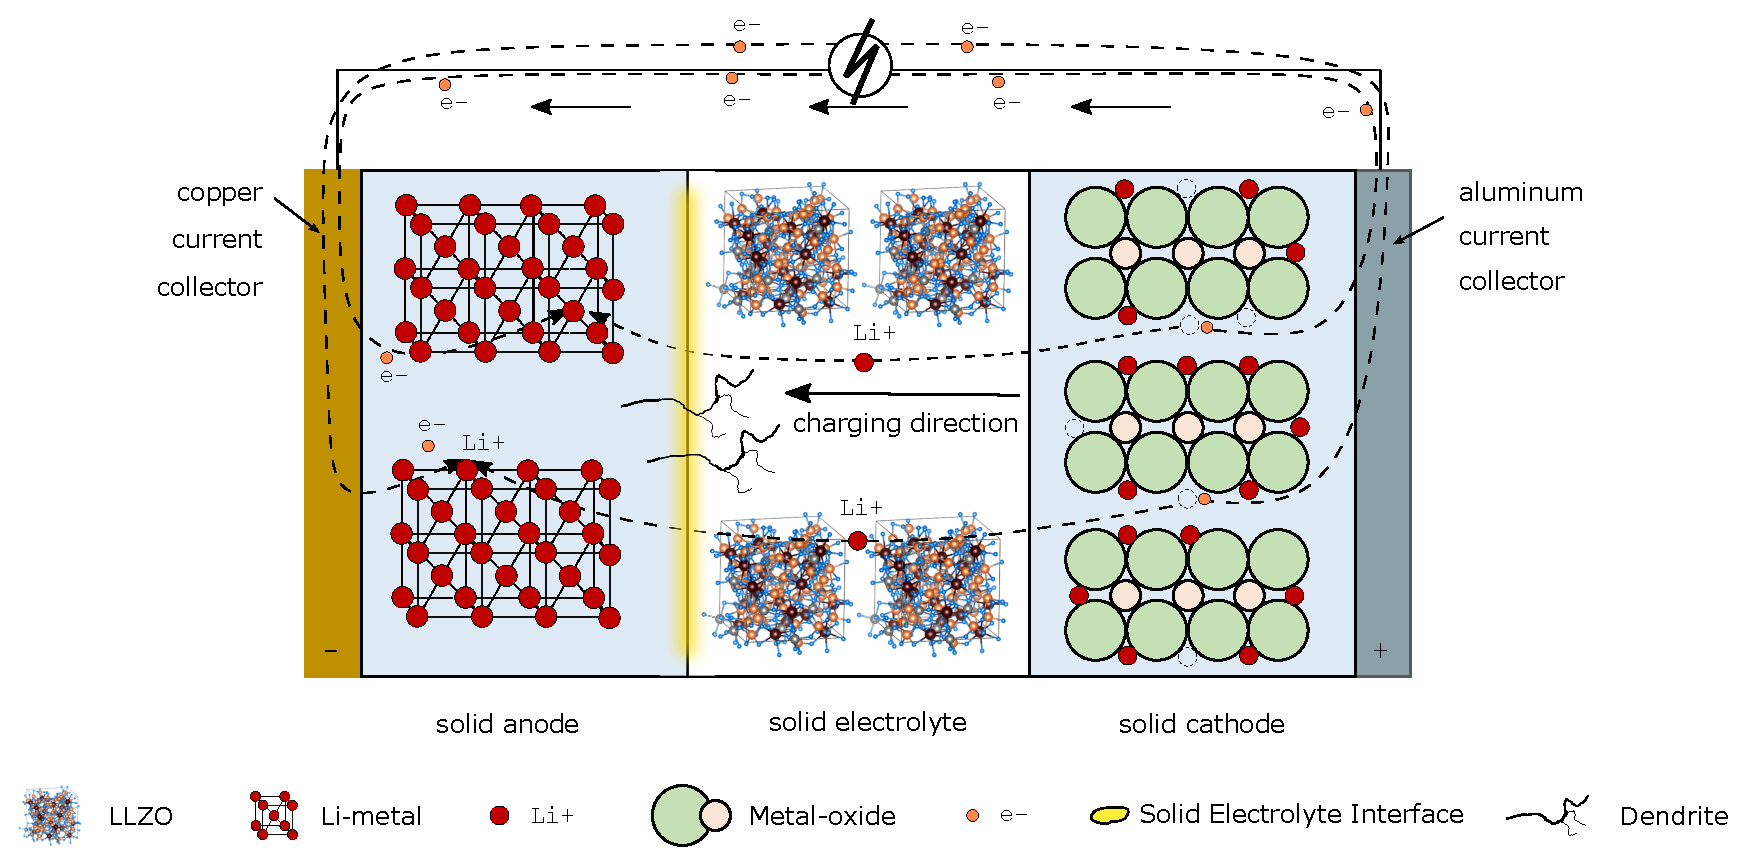
\includegraphics[width=28cm]{./figs/transport/transporttext}}\vspace*{1em}
	% 			%       \newcaption{0.8\colwidth}{Dendrite formation: After a several number of charging cycles, dendrite branches are slowly formed and developed from Solid electrolyte interface (SEI) through grain boundaries.}
	% 		    %   \end{center}
	% 	\end{itemize}
	% }
\end{columns}
% ---------------------------------------------------------------------------------------------------------------- %
\block{Nucleation interface: Taking place at the critical dendritic interface}{
	\begin{minipage}{0.45\textwidth}
		% Nucleation interface: Taking place at the critical dendritic interface (SE|SSE)
		\begin{align*}
			 & \rho\,
			\partial^2_{t^2}
			\bm{u}^{(s)}
			+
			\nabla \cdot
			\Big(
			\accentset{\scriptstyle 4}{\mathbb{C}}^{f^{\mathbb{D}(\Omega)}_{(\lambda,\mu)}}
			:\nabla\Bu^{(s)}
			\Big)
			+
			\rho\nabla V_{e}
			= \textbf{0},                                                                                                                                                                                                                                                               \\
			%--------------------------------
			\text{s.t.}\quad
			 & a_{\text{Griffith}} := a^{*} = \arg\min_{a\in\mathbb{R}}{\bigintsss\!\!\!\!\!\!\bigintsss\!\!\!\!\!\!\bigintsss_{\Omega} f(a,\bm{u};\lambda,\mu,\bm{d}\otimes\bm{d}) \, d\Omega - \bigintsss\!\!\!\!\!\!\bigintsss_{\Gamma} f(a;\gamma) \, d\Gamma}\Bigg|_{\bm{u}^{(s)}}
		\end{align*}
		\begin{align*}
			 & \rho\,
			\partial^2_{t^2}
			\bm{u}^{(s)}
			+
			\nabla \cdot
			\Big(
			\accentset{\scriptstyle 4}{\mathbb{C}}^{f^{\mathbb{D}(\Omega)}_{(\lambda,\mu)}}
			:\nabla\Bu^{(s)}
			\Big)
			+
			\rho\nabla V_{e}
			= \textbf{0},                                                                                                                                                                                                                                                               \\
			%--------------------------------
			\text{s.t.}\quad
			 & a_{\text{Griffith}} := a^{*} = \arg\min_{a\in\mathbb{R}}{\bigintsss\!\!\!\!\!\!\bigintsss\!\!\!\!\!\!\bigintsss_{\Omega} f(a,\bm{u};\lambda,\mu,\bm{d}\otimes\bm{d}) \, d\Omega - \bigintsss\!\!\!\!\!\!\bigintsss_{\Gamma} f(a;\gamma) \, d\Gamma}\Bigg|_{\bm{u}^{(s)}}
		\end{align*}
		\begin{align*}
			 & \rho\,
			\partial^2_{t^2}
			\bm{u}^{(s)}
			+
			\nabla \cdot
			\Big(
			\accentset{\scriptstyle 4}{\mathbb{C}}^{f^{\mathbb{D}(\Omega)}_{(\lambda,\mu)}}
			:\nabla\Bu^{(s)}
			\Big)
			+
			\rho\nabla V_{e}
			= \textbf{0},                                                                                                                                                                                                                                                               \\
			%--------------------------------
			\text{s.t.}\quad
			 & a_{\text{Griffith}} := a^{*} = \arg\min_{a\in\mathbb{R}}{\bigintsss\!\!\!\!\!\!\bigintsss\!\!\!\!\!\!\bigintsss_{\Omega} f(a,\bm{u};\lambda,\mu,\bm{d}\otimes\bm{d}) \, d\Omega - \bigintsss\!\!\!\!\!\!\bigintsss_{\Gamma} f(a;\gamma) \, d\Gamma}\Bigg|_{\bm{u}^{(s)}}
		\end{align*}
		\begin{align*}
			 & \rho\,
			\partial^2_{t^2}
			\bm{u}^{(s)}
			+
			\nabla \cdot
			\Big(
			\accentset{\scriptstyle 4}{\mathbb{C}}^{f^{\mathbb{D}(\Omega)}_{(\lambda,\mu)}}
			:\nabla\Bu^{(s)}
			\Big)
			+
			\rho\nabla V_{e}
			= \textbf{0},                                                                                                                                                                                                                                                               \\
			%--------------------------------
			\text{s.t.}\quad
			 & a_{\text{Griffith}} := a^{*} = \arg\min_{a\in\mathbb{R}}{\bigintsss\!\!\!\!\!\!\bigintsss\!\!\!\!\!\!\bigintsss_{\Omega} f(a,\bm{u};\lambda,\mu,\bm{d}\otimes\bm{d}) \, d\Omega - \bigintsss\!\!\!\!\!\!\bigintsss_{\Gamma} f(a;\gamma) \, d\Gamma}\Bigg|_{\bm{u}^{(s)}}
		\end{align*}
		\begin{align*}
			 & \rho\,
			\partial^2_{t^2}
			\bm{u}^{(s)}
			+
			\nabla \cdot
			\Big(
			\accentset{\scriptstyle 4}{\mathbb{C}}^{f^{\mathbb{D}(\Omega)}_{(\lambda,\mu)}}
			:\nabla\Bu^{(s)}
			\Big)
			+
			\rho\nabla V_{e}
			= \textbf{0},                                                                                                                                                                                                                                                               \\
			%--------------------------------
			\text{s.t.}\quad
			 & a_{\text{Griffith}} := a^{*} = \arg\min_{a\in\mathbb{R}}{\bigintsss\!\!\!\!\!\!\bigintsss\!\!\!\!\!\!\bigintsss_{\Omega} f(a,\bm{u};\lambda,\mu,\bm{d}\otimes\bm{d}) \, d\Omega - \bigintsss\!\!\!\!\!\!\bigintsss_{\Gamma} f(a;\gamma) \, d\Gamma}\Bigg|_{\bm{u}^{(s)}}
		\end{align*}
		Therefore
		\begin{align*}
			\therefore\quad
			\boxed{
			a_{\text{Griffith}} := a^{*} = \arg\min_{a\in\mathbb{R}}{\bigintsss\!\!\!\!\!\!\bigintsss\!\!\!\!\!\!\bigintsss_{\Omega} f(a,\bm{u};\lambda,\mu,\bm{d}\otimes\bm{d}) \, d\Omega - \bigintsss\!\!\!\!\!\!\bigintsss_{\Gamma} f(a;\gamma) \, d\Gamma}\Bigg|_{\bm{u}^{(s)}}
			}
		\end{align*}
		\begin{center}
			% \inputfig{floats/dendrite_pdirection_battonly}{dendrite_pdirection_battonly}
			% \inputfig{floats/routine_woTV_spectral}{routine_woTV_spectral}
		\end{center}
	\end{minipage}
	\hfill
	\begin{minipage}{0.55\textwidth}
		% Distribution of the analytical maximal shear stress component $\WAsigma^{\Pi}_{x_1x_2}$, 
		% around the crack tip $a_{c}$.
		Boundary settings
		\begin{center}
			\inputfig{floats/structuraltwofields}{structuraltwofields}
			% 	\inputfig{floats/maxshear_9figs_456}{maxshear_9figs_456}
		\end{center}
		The set of boundary conditions is likewise the path of the pressure-centric dendritic crack.\\
		\begin{center}
			\inputfig{floats/routine_woTV_numa_one}{routine_woTV_numa_one}
		\end{center}
		Comparison: Analytical vs. Numerical solutions
		\begin{center}
			\inputfig{floats/comparison_ana_numa}{comparison_ana_numa}
		\end{center}
		% \begin{minipage}{0.45\textwidth}
		% 	\begin{center}
		% 		\inputfig{floats/routine_woTV_numa}{routine_woTV_numa}
		% 	\end{center}
		% \end{minipage}
		% \hfill
		% \begin{minipage}{0.45\textwidth}
		% 	\begin{center}
		% 		\inputfig{floats/routine_woTV_numa}{routine_woTV_numa}
		% 	\end{center}
		% \end{minipage}
	\end{minipage}
	% \begin{center}
	% 	\inputfig{floats/routine_woTV}{routine_woTV}
	% \end{center}
	% Nucleation interface: Taking place at the critical dendritic interface (Solid electrode | Solid-state electrolyte)
}
\begin{columns}
	\column{0.14}
	% ---------------------------------------------------------------------------------------------------------------- %	
	\block{Contact}{
		% {
		% 		\raggedleft
		% 		\begin{tikzpicture}
		% 			\node (qrcode) {\inputfig{floats/QRcode_ACoM}{QRcode_ACoM}};
		% 			\node[left= 0mm of qrcode.north west, yshift=-15mm] {Tuan Vo};
		% 			% \node[left= 0mm of qrcode.north west, yshift=-40mm] {Applied and Computational Mathematics (ACoM)};
		% 			% \node[left= 0mm of qrcode.north west, yshift=-55mm] {RWTH Aachen University};
		% 			\node[left= 0mm of qrcode.north west, yshift=-30mm] {vo@acom.rwth-aachen.de};
		% 		\end{tikzpicture}
		% 	}
		\begin{center}
			\inputfig{floats/QRcode_ACoM_Email}{QRcode_ACoM_Email}
		\end{center}
		% \inputfig{floats/QRcode_ACoM}{QRcode_ACoM}
		% Tuan Vo $\cdot$ RWTH Aachen University $\cdot$ Email: vo@acom.rwth-aachen.de
	}
	\column{0.86}
	%---------------------------------------------------------------------------------------------------------------- %	
	\block{References}{
		\vspace*{-3em}
		\renewcommand{\refname}{~}
		\begin{thebibliography}{2}
			\bibitem{vo2018}
			\textbf{T.Vo},
			\!\!
			\emph{Modeling\! the\! swelling\! phenomena\! of\! li-ion\! batt.\!
				cells\! based\! on\! a\! numerical\! chemo-mech.\! coupled\! approach}.
			MA, Robert Bosch Battery Systems GmbH, 2018.
			
			\bibitem{braun2015}
			\textbf{S.Braun},\! C.Yada\! and A.Latz,
			\!\!\!\!
			\emph{Thermodynamically\! consistent\! model\! for\!
				Space-Charge-Layer\! formation\! in\! a\! solid\! electrolyte}.
			Jr.\! Phys.\! Chem.,\! 119,\! 22281-22288,\! 2015.
			
			\bibitem{hueter2017}
			\textbf{C.Hüter}, S.Fu, M.Finsterbusch, E.Figgemeier, L.Wells, and R.Spatschek,
			\emph{Electrode-electrolyte interface stability in solid state electrolyte system:
				influence of coating thickness under varying residual stresses}. 
			AIMS materials Science, 4(4):867-877, 2017.
			
			\bibitem{kim2022}
			\textbf{S.Kim}, 
			J.S.Kim, L.Miara, Y.Wang, S.K.Jung, S.Y.Park, Z.Song, 
			H.King, M.Badding, J.M.Chang, V.Roev, G.Yoon, R.Kim, J.H.Kim, K.Yoon, D.Im, and K.Kang,
			\emph{High-energy and durable li metal batt. using garnet-type
				solid electrolytes with tailored li-metal compatibility}.
			Nature Communications, 13(1):1883, 2022.
			% $(*)$ (Solid electrode | Solid-state electrolyte)
		\end{thebibliography}
	}
\end{columns}
\block{}{
	\vspace{-0.6em}
	\begin{minipage}{0.2\textwidth}
		\begin{center}
			
\includegraphics[width=0.99\textwidth]{./floats/logos/siam.eps}
		\end{center}
	\end{minipage}
	\hfill
	\begin{minipage}{0.2\textwidth}
		\begin{center}
			
\includegraphics[width=0.6\textwidth]{./floats/logos/siamcse23.eps}
		\end{center}
	\end{minipage}
	\hfill
	\begin{minipage}{0.2\textwidth}
		\begin{center}
			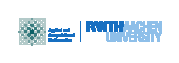
\includegraphics[width=0.99\textwidth]{./floats/logos/acomrwth.eps}
		\end{center}
	\end{minipage}
	\hfill
	\begin{minipage}{0.2\textwidth}
		\begin{center}
			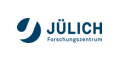
\includegraphics[width=0.6\textwidth]{./floats/logos/fzj.eps}
		\end{center}
	\end{minipage}
	\vspace{-0.6em}
	% 
\includegraphics[width=0.3\textwidth]{./floats/logos/siam_siamcse23_acomrwth_fzj.eps}
}
% ---------------------------------------------------------------------------------------------------------------- %	
% \block{References}{
% 	\vspace*{-3em}
% 	\renewcommand{\refname}{~}
% 	\begin{thebibliography}{2}

% 		\bibitem{viozat1997implicit}
% 		\textbf{T. Vo} \emph{Modeling the swelling phenomena of li-ion battery
% 			cells based on a numerical chemo-mechanical coupled approach}. 
% 		Master thesis, Robert Bosch Batteries Systems GmbH, 2018.

% 		\bibitem{braun2015SCL}
% 		\textbf{S. Braun}, C. Yada and A. Latz. \emph{Thermodynamically consistent model for
% 			Space-Charge-Layer formation in a solid electrolyte}. 
% 		Journal of Physical Chem., 119, 22281-22288, 2015.

% 		\bibitem{hueter2017}
% 		\textbf{C. Hüter}, S. Fu, M. Finsterbusch, E. Figgemeier, L. Wells, and R. Spatschek. 
% 		Electrode-electrolyte interface stability in solid state electrolyte system: 
% 		influence of coating thickness under varying residual stresses. 
% 		AIMS materials Science, 4(4):867-877, 2017.

% 		\bibitem{kim2022}
% 		\textbf{S. Kim}, J. S. Kim, L. Miara, Y. Wang, S. K. Jung, S. Y. Park, Z. Song, 
% 		H. King, M. Badding, J. M. Chang, V. Roev, G. Yoon, R. Kim, J. H. Kim, K. Yoon, D. Im, 
% 		and K. Kang. “High-energy and durable lithium metal batteries using garnet-type 
% 		solid electrolytes with tailored lithium-metal compatibility,” 
% 		Nature Communications, 13(1):1883, Apr 2022.
% 		% $(*)$ (Solid electrode | Solid-state electrolyte)
% 	\end{thebibliography}
% }
\end{document}
% ---------------------------------------------------------------------------------------------------------------- %